\documentclass{szzclass}

\usepackage{amsmath}
\usepackage{graphics}

% spacing
\usepackage{titlesec}
% \titlespacing*{\section}{0pt}{1ex}{0.5ex}
\titlespacing*{\subsection}{0pt}{1ex}{0ex}

\title{Základní pojmy teorie grafů. \\
\large Grafové algoritmy:   procházení grafu do šířky a do hloubky, určení souvislých komponent,   topologické uspořádání, vzdálenosti v grafech, konstrukce minimální kostry a nejkratších cest v ohodnoceném grafu.}

\renewcommand*\contentsname{Obsah}

\begin{document}
\maketitle

\tableofcontents
\newpage

\section{Základní pojmy}

\subsection{Graf}

\textbf{Neorientovaný graf je uspořádaná dvojice ($V, E$)}, kde
\begin{itemize}
    \item V je neprázdná konečná množina vrcholů,
    \item E je množina hran.
\end{itemize}

\textbf{Množina všech možných hran: $\binom{V}{2}$.}\newline
Platí tedy $E \subseteq \binom{V}{2} \subseteq 2^V$, kde $2^V$ je množina všech podmnožin množiny~V.

\textbf{Nechť $G$ je graf.} Pak:
\begin{itemize}
    \item $V(G)$ značí jeho množinu vrcholů a $|V(G)|$  velikost této množiny
    \item $E(G)$ značí jeho množinu hran a $|E(G)|$  velikost této množiny
\end{itemize}

Dále, \textbf{nechť $e = \{u, v\}$ je hrana grafu G.} Pak:
\begin{itemize}
    \item $u$ a $v$ jsou \textbf{koncové vrcholy}
    \item oba koncové body jsou si na grafu $G$ navzájem \textbf{sousedy}
    \item oba koncové body jsou \textbf{incidentní} s hranou $e$
\end{itemize}

\subsection{Doplněk}
\textbf{Doplěk} $\overline{G}$ grafu $G = (V, E)$ je graf $(V, \binom{V}{2} \backslash E)$.

\begin{figure}[h]
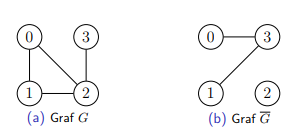
\includegraphics[width=0.5\textwidth]{topics/bi-spol-4/images/doplnek.png}
\end{figure}


\subsection{Isomorfismus}
Grafy $G$ a $H$ jsou \textbf{isomorfní}, právě tehdy, když existuje zobrazení $f:V(G)~\rightarrow~V(H)$, kde $f$ je bijekce a pro každou dvojici vrcholů $u$ a $v$ z $V(G)$ platí, $\{u,v\} \in E(G)$ právě tehdy, když $\{f(u), f(v)\} \in E(H)$.

\textbf{Automorfismus} grafu $G$ je isomorfismus, grafu $G$ se sebou samým. (ukazuje symetrie grafu)

\subsection{Vrcholy}

\textbf{Stupeň} vrcholu $v$ v grafu $G$ je počet hran, které vrchol $v$ obsahují a značíme jej $deg_G(v)$.

\textbf{Otevřené okolí} vrcholu $v$ v grafu $G$ je množina všech sousedů vrcholu $v$ a značíme jej $N_G(v$).

\textbf{Uzavřené okolí} vrcholu $v$ v grafu $G$ je $N_G(v) \cup \{v\}$ a značíme jej $N_G[v]$.

\textbf{Regulární graf}, je graf, ve kterém mají všechny vrcholy stejný stupeň.

\textbf{Princip sudosti} $\sum_{v \in V} deg_G(v) = 2|E|$

\subsection{Podgraf}
Graf $H$ je \textbf{podgrafem} grafu $G$, když $V(H) \subseteq V(G)$ a
$E(H) \subseteq E(G)$; tuto skutečnost značíme $H \subseteq G$.

Graf $H$ je \textbf{indukovaným podgrafem} grafu $G$, když $V(H) \subseteq V(G)$ a $E(H) = E(G) \cap \binom{V(H)}{2}$; tuto skutečnost značíme $H \leq G$.



\begin{figure}[h]
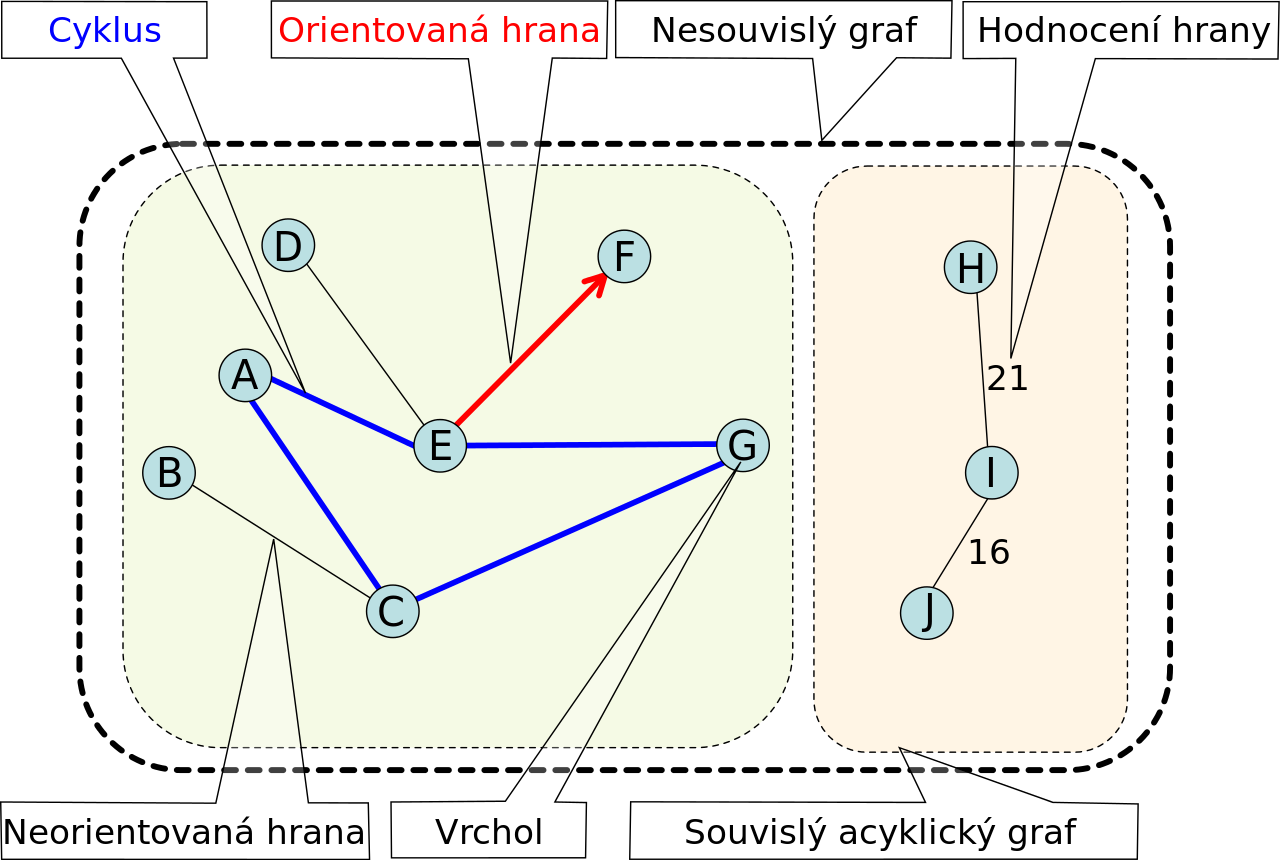
\includegraphics[width=0.95\textwidth]{topics/bi-spol-4/images/graf.png}
\end{figure}


\newpage

\section{Typy grafů}
\subsection{Uplný graf $K_n$}
\textit{Graf, kde jsou všechny vrcholy spojeny hranou se všemi ostatními vrcholy.}

\textbf{Nechť $n \geq 1$.\newline
Úplný graf na n vrcholech $K_n$ je graf ($V, \binom{V}{2}$), kde $|V| = n$.}

\subsection{Úplný $k$-partitní graf}
\textit{Graf, rozdělený na $k$ skupin, kde je každý vrchol spojen hranou se všemi vrcholy ze všech ostatních skupin, ale není spojen s žádným vrcholem ze své vlastní skupiny.}

\textbf{Nechť $\forall i ∈ \{1, . . . k\} : n_i \geq 1$.\newline
Úplný $k$-partitní graf $K_{n1,n2,...,nk}$
je graf ($\cup^k _{i=1} V_i, E),$\newline kde $\forall i, j ∈ \{1, . . . , k\}, i \neq j : V_i \cap V_j = ∅, |V_i| = n_i$\newline
a $E = \{\{x, y\} | \exists i, j \in \{1, . . . , k\}, i \neq j : x ∈ V_i, y ∈ V_j\}$,\newline
neboli $E = \binom{ \cup^k_{i=1} V_i}{2} \backslash \cup^k_{i=1} \binom{V_i}{2}$.
}

\subsection{Cestat $P_m$}
\textit{Graf, který má $m$ hran, $m+1$ vrcholů a tvoří cestu.}

\textbf{Nechť $m \geq 0$.\newline
Cesta délky $m$} (s $m$ hranami) \textbf{$P_m$ je graf\newline
($\{0, . . . , m\}, \{\{i, i + 1\} | i \in \{0, . . . ,m-1\}\}$).
}

\subsection{Kružnice $C_n$}
\textit{Graf, který ma $n$ vrcholů i hran a na všechny vrcholy navazují právě dvě hrany.}

\textbf{Nechť $n \geq 3$.\newline
Kružnice délky $n$ $C_m$ je graf\newline
($\{1, . . . , n\}, \{\{i, i + 1\} | i \in \{1, . . . ,n-1\}\} \cup \{\{1, n\}\}$).
}

\subsection{Hvězda $S_n$}
\textit{Uplný bipartitní graf, kde je v první partitě právě jeden vrchol a ve druhé alespoň jeden vrchol.}

\textbf{Nechť $n \geq 1$.\newline
Hvězda s $n$ paprsky $S_n$ je graf $K_{1,n}$.
}


\section{Procházení grafu}

\subsection{Vzdálenost}
Vzdálenost $d(u, v)$ dvou vrcholů $u$ a $v$ v (orientovaném) grafu $G$ je
délka nejkratší (orientované) cesty v $G$ z vrcholu $u$ do vrcholu $v$.
Pokud z $u$ do $v$ žádná cesta neexistuje, definujeme $d(u, v) = \inf$.


\subsection{DFS}
\textit{Prohledávání do hloubky}

\begin{figure}[h!]
\begin{verbatim}
Algoritmus DFS_graf (graf G, vrchol v):
(1) pro každý vrchol u ∈ V (G):
(2)     stav(u) := nenalezený
(3) DFS(v)

DFS (vrchol v):
(4) Když stav(v) není nenalezený
(5)     return
(6) stav(v) := otevřený
(7) Pro každého souseda u vrcholu v:
(8)     DFS(u)
(9) stav(v) := uzavřený
    
\end{verbatim}
\end{figure}


\subsection{BFS}
\textit{Prohledávání do šířky}

\begin{figure}[h!]
\begin{verbatim}
Algoritmus BFS(G, s):
(1) pro každý vrchol v ∈ V (G):
(2)     stav(v) := nenalezený
(3)     D(v) := P(v) := undef
(4) stav(s) := otevřený
(5) D(s) := 0
(6) Q := fronta obsahující s
(7) Dokud je fronta Q neprázdná:
(8)     Odeber začátek fronty Q, označ ho v
(9)     Pro všechny sousedy w vrcholu v:
(10)        Pokud stav(w) = nenalezený:
(11)        stav(w) := otevřený
(12)        D(w) := D(v) + 1
(13)        P(w) := v
(14)        přidej w do fronty Q
(15)    stav(v) := uzavřený
\end{verbatim}    
\end{figure}

\section{Souvislost}
\subsection{Souvislý graf}
Graf $G$ je \textbf{souvislý}, pokud pro každé dva vrcholy $u$, $v$ v grafu $G$ existuje $u$-$v$-cesta.

\subsection{Souvislá komponenta}
Indukovaný podgraf $H$ grafu $G$ je souvislou komponentou, pokud je souvislý a neexistuje žádný souvislý podgraf $F$, $F \neq H$, grafu $G$ takový, že $H \subseteq F$.
(Souvislá komponenta je tedy v inkluzi maximální souvislý podgraf grafu $G$).

\section{Topologické uspořádání grafu}
\subsection{Definice}
Topologické uspořádání orientovaného acyklického grafu $G = (V, E)$ je takové pořadí vrcholů $v_1, v_2, . . . , v_n$ grafu $G$, že pro každou hranu $(vi, vj) \in E$ platí $i~<~j$.

\subsection{TopSort}
\begin{figure}[h!]
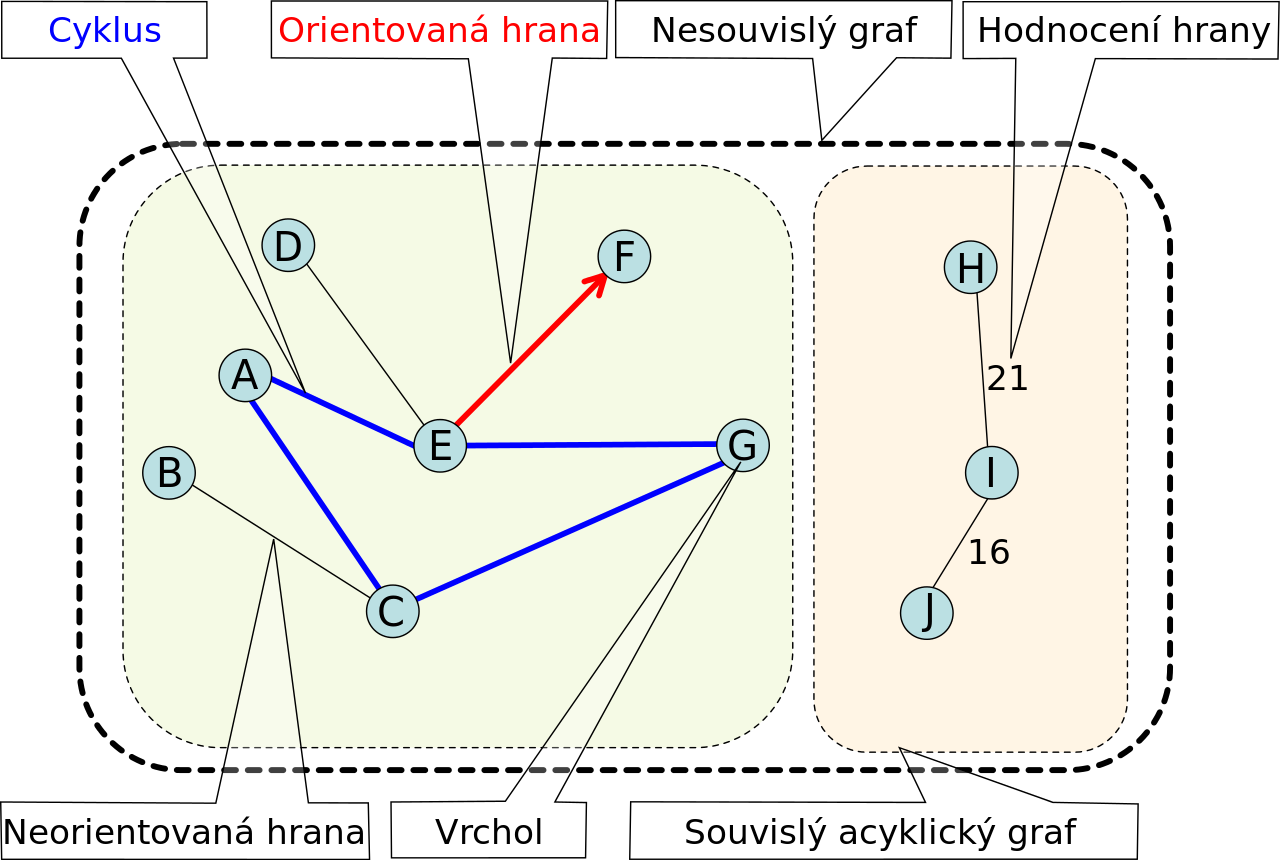
\includegraphics[width=0.95\textwidth]{topics/bi-spol-4/images/graf.png}   
\end{figure}

\section{Ohodnocený graf}
\subsection{Minimální kostra}
Nechť $G = (V , E)$ je souvislý neorientovaný graf a $w : E \rightarrow R$
váhová funkce, která přiřazuje hranám čísla – jejich váhy.
Váhovou funkci můžeme přirozeně rozšířit na podgrafy:
Váha $w(H)$ podgrafu $H \subseteq G$ je součet vah jeho hran.
Kostra je minimální, pokud má mezi všemi kostrami nejmenší
váhu.

\begin{figure}[h!]
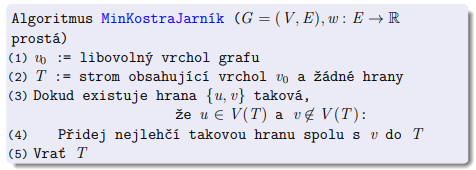
\includegraphics[width=0.8\textwidth]{topics/bi-spol-4/images/jarnik.png}
\end{figure}

\begin{figure}[h!]
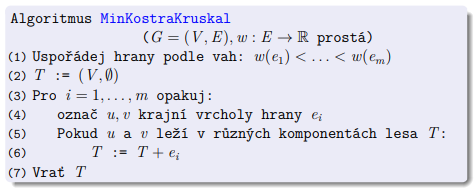
\includegraphics[width=0.8\textwidth]{topics/bi-spol-4/images/kruskal.png}
\end{figure}

\newpage

\subsection{Hledaní nejkratšíí cesty}
\textit{\textbf{Dijkstrův}: předpokládá nezáporné ohodnocení hran}

\textit{\textbf{Bellmanův-Fordův}: předpokládá neexistenci záporných cyklů v grafu}

\begin{figure}[h!]
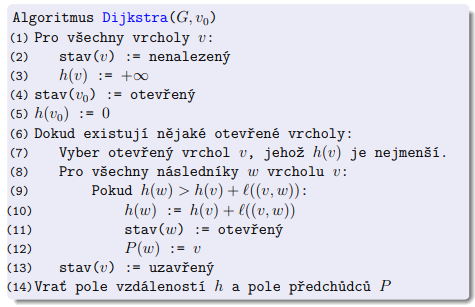
\includegraphics[width=0.8\textwidth]{topics/bi-spol-4/images/dijkstra.png}
\end{figure}


\begin{figure}[h!]
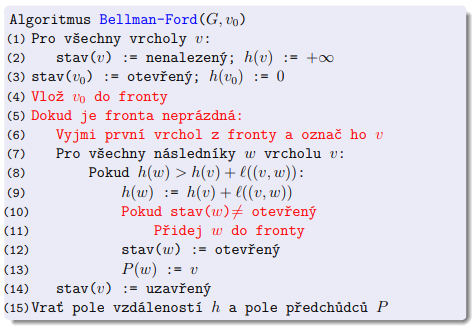
\includegraphics[width=0.8\textwidth]{topics/bi-spol-4/images/bellman-ford.png}
\end{figure}


\end{document}